%!TEX program=xelatex
\documentclass[UTF8]{ctexart}

%%%%%% 导入包 %%%%%%
\usepackage{graphicx}
\usepackage{xcolor}
\usepackage{tabularx}
\usepackage{algorithm,algorithmicx}
\usepackage{algpseudocode}
\usepackage{amsmath,amssymb,amsthm}

%%%%%% 算法部分改为中文显示 %%%%%%%%%
\floatname{algorithm}{算法}
\renewcommand{\algorithmicrequire}{\textbf{输入:}}
\renewcommand{\algorithmicensure}{\textbf{输出:}}

%%%% 正文开始 %%%%
\begin{document}

\title{第二次大作业}
%
\author{徐维震\quad 陈文宇\quad 刘小端\quad 高鹏智\quad 阴雅萱}

\date{\today}

\maketitle{}
\begin{abstract}
	本文借助最小二乘法、牛顿迭代法解决了给定点组的四次多项式最小二乘拟合与非线性函数在局部上的最小二乘拟合问题。并且基于牛顿迭代法给出了关于全局最优解的思考,同时使用退火模拟算法进行了验证。
\end{abstract}

\newpage
\tableofcontents
\newpage

\section{问题重述与同类问题回顾}


已给定一组离散点$(x_{i},y_{i})$如下:\\
\begin{table}[h]
	\centering
	\resizebox{\textwidth}{!}{	
		\begin{tabular}{cccccccccccc}
			\hline
			x&-1&-0.8&-0.6&-0.4&-0.2&0.0&0.2&0.4&0.6&0.8&1.0\\
			\hline
			y&-0.8669&-0.2997&0.3430&1.0072&1.6416&2.2202&2.6558&2.9823&3.1755&03.2416&3.1974\\
			\hline
	\end{tabular}}
	\caption{离散点组}
\end{table}


问题重述如下:\\
接下来希望利用四次多项式F(x)与含有三角函数的非线性函数G(x)给出两种对于同一组点的最小二乘拟合,并给出两拟合的最小误差
$\epsilon_{1},\epsilon_{2}$。\\
在这里,不妨回顾《数值分析》:\\
现有观测数据$(x_{i},y_{i})$,$i = 0,1,2...,N$,N为样品点数目,设:
$$f(x)=\sum^{m}_{i=0}a_{i}x^{i},N>>m$$
原题求解方法如下:\\
令Q为平方逼近的偏差值:\\
$$Q(a_{0},a_{1},a_{2},\dots,a_{m})=\sum^{m}_{i=1}(y_{i}-a_{0}-a_{1}x_{i}-\dots-a_{m}x_{i}^{m})^{2}$$
该问题转化为求解$a_{0},a_{1},a_{2},a_{3},a_{4}$,使得偏差Q取极小值。\\
注意到$a_{i}\textrightarrow+\infty$时,$Q\textrightarrow+\infty$,
又因为Q为$a_{0},a_{1},a_{2},\dots,a_{m}$的连续函数,故问题必存在解。
设其解为$a_{0}^{*},a_{1}^{*},a_{2}^{*},\dots,a_{m}^{*}$,则其满足:
$$\frac{\partial Q}{\partial a_{i}}(a_{0}^{*},a_{1}^{*},a_{2}^{*},\dots,a_{m}^{*}) = 0,i=0,1,\dots,m$$
由此得法方程组。然后求解法方程组如下:
\[
s_{k}=\sum_{i=0}^{N}x_{i}^{k},u_{k}=\sum_{i=0}^{N}y_{i}x_{i}^{k}
\]
\[
\\
\left\{
\begin{aligned}
	&s_{0}a_{0}+s_{1}a_{1}+\dots+s_{m}a_{m}  &=u_{0}\\
	&s_{1}a_{0}+s_{1}a_{1}+\dots+s_{m+1}a_{m}&=u_{1}\\
	\vdots&\qquad\qquad\qquad\vdots&\vdots\\
	&s_{m}a_{0}+s_{m+1}a_{1}+\dots+s_{2m}a_{m}&=u_{m}\\
\end{aligned}
\right.
\]


可得$a_{0},a_{1},a_{2},\dots,a_{m}$,最后由题目误差表达式:
$$\epsilon=(\sum_{i=0}^{10}(p(x_i)-f(x_{i})))^{\frac{1}{2}}$$
求解拟合误差$\epsilon$并输出多项式系数。


\section{利用四次多项式进行最小二乘拟合结果}
不妨由上述解法进行四次多项式最小二乘拟合,直接代入题目参数,
令m=4,N=10,然后照图索骥。由多项式基底的线性无关性质易知满足哈尔条件,即该基底拟合多项式结果是唯一的。\\
拟合源码详见附录I,最后得到保留六位有效数字的拟合结果:
$$f(x)=2.20128+2.54703x-1.33325x^{2}-0.516217x^{3}+0.297549x^{4}$$
$$\epsilon=0.006074$$

\section{对非线性方程的牛顿迭代法结果}
由参考文献\cite{Yan2004}的牛顿迭代法记载,我们采用了如下迭代格式:
\[
\left\{
\begin{aligned}
	&a^{k+1}=a^{k}+\bigtriangleup^{k}
	\\
	&F'(a^{k}) \bigtriangleup^{k} + F(a^{k})=0
\end{aligned}
\right.
\]         

其中$a=(a_{0},a_{1},a_{2},a_{3},a_{4})$ 为所求系数向量,上角标为迭代次数,$F’$为代码中的Jacobi矩阵。
由牛顿法的局部收敛性定理\footnote{参见《非线性数值分析》Page53,定理3.2},可知\quad 如果Jacobi矩阵可逆,
我们的求解过程必定有解。
迭代法代码详见源代码II,最后我们得到迭代收敛的数值为:\\
$$f(x)=1.33+2.23sin(1.15x)+0.874cos(1.76x)$$
$$\epsilon=0.010010$$

由此只用六步即收敛至的足够的精度用于保留三位有效数字,可以说这一迭代是十分有效的。
Newton迭代法保证了收敛点是极值点,而简单地比较该点与附近点函数值大小可知所求点是极小值点。

\section{利用模拟退火算法全局搜索极小值验证结果}
观察$\epsilon=(\sum_{i=0}^{n}(p(x_{i})-f(x_i)^{2})^\frac{1}{2}$函数,可知
对于给定的$a_{2},a_{4}$,$p(x)$是基于基函数$1,sin(a_{2}x),cos(a_{4}x)$的对于$f(x)$的最小二乘法拟合函数,
所以可以利用最小二乘法求解$a_{0},a_{1},a_{3}$。
任意给定初始矩形域$a_{2}\times a_{4}=[\aleph_{1},\beta_{1}]\times[\aleph_{2},\beta_{2}]$,
取其中点作为迭代点$i$(初始状态),四个顶点中函数值最小者作为比较点(过渡状态),
若迭代点函数值大于比较点函数值,则接受比较点和迭代点连线的中点$j$作为新的迭代点,
否则迭代点更新以如下概率接受:
$$e^{\dfrac{\epsilon_{i}-\epsilon_{j}}{T_{0}}}$$
其中$T0$为温度,一般地我们采用$T_{0}=0.99\times T_{0}$进行退火。
上述过程详见源代码\oldstylenums{3}:模拟退火算法。

由于函数关于$a_[2],a_[4]$具有周期性,可以推测,当初始矩形域不同时,上述代码运行结果很有可能是不一样的,
但是这些运行结果可以保证函数值相同,且均与牛顿迭代法运行结果对应的函数值相等。
对于以$(0,0)$为中心,边长为依次为20、200、2000的方形域和$T_{0}$对应10,100,1000 的结果展示如下:
\begin{figure*}[h!]
	\centering
	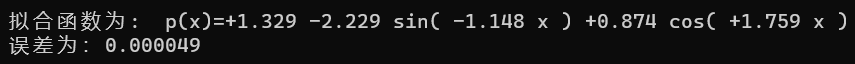
\includegraphics[width=10cm,height=0.7cm]{figure1}
	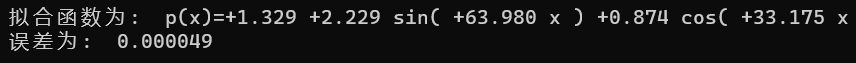
\includegraphics[width=10cm,height=0.7cm]{figure2}
	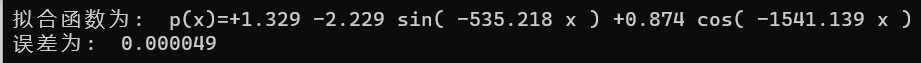
\includegraphics[width=10cm,height=0.7cm]{figure3}
\end{figure*}

上述结果充分说明了牛顿迭代法结果是近似值附近的极小值点。

\section{关于全局最优解思考}
第二题中我们小组基于足够好的初值使用牛顿迭代法一次性地得出了想要的结果。但是如果初值不太好,我们得到的解点也许不是最小值点。不过对于该函数而言,函数值在$a_[0],a_[1],a_[3]$的绝对值趋于无穷时趋于无穷,并且关于$a_[2],a_[4]$具有周期性,所以可以将目标点限制在有限立方体内。将这个立方体分为多个小立方体,分别在小立方体内部取点作为牛顿迭代法的初值,比较函数在求出点处的值,得到最小值点。

\section{结语}
在最小二乘拟合的过程中,不同函数初始结构的给定,会影响算法的给定,在四次多项式拟合中可以直接按照教材求解法方程组的方案来给定未知参数值,而在含有三角函数的非线性函数中,采取了牛顿迭代法经过6步下降即终止迭代、取得了显著的计算量优化。
\footnote[1]{在利用Newton下降法之前也尝试了求解类似第一部分求解方案的法方程组,在附录III中给出了一个最小二乘法的验证程序。但是相同精度下,需要计算量过大,于是只作为验证。}
但是在牛顿迭代法后的验证仍必不可少,以保证求解到的极值点是最值点。因为缺少验证的情形下,取梯度为0的情况不一定为所求情形。
\footnote[2]{比如鞍点,数学分析中不乏类似反例。}
所以、我们需要更加细致地掌握函数的性质,并依靠拟合点观察选择恰当的拟合函数形式与拟合手法,在同等误差限下优化算法计算量,以方便同类方法的推广应用。

\newpage
\begin{thebibliography}{99}
	\bibitem{Yan2004}{黄明游,冯果忱主编. 数值分析.下册 北京: 高等教育出版社, 2008.1.}
	\bibitem{Ma2022}{黄象鼎,曾钟钢,马亚南编著.非线性数值分析.武汉大学出版社}
\end{thebibliography}

\section{附录}

\subsection{源代码\oldstylenums{1}:四次多项式拟合}

\begin{verbatim}
#include <stdio.h>
#include <stdlib.h>
#include <math.h>
double least_square(int n, double *x, double *y, int m, double *a);
void assemble_matrix(int n, double *x, int m, double **A);
void right_side(int n, double *x, double *y, int m, double *b);
void basis_function(int n, double *x, int i, double *phi_i);
double dot(int n, double *vector1, double *vector2);
void output(int n, int m,double *x, double *y, 
		double *a,double xs, double ys,double e); 
void ColElim(int n, double **A, double *b, double *x);
double compute_value(int m, double *a, double xs);
int main(){
	/*
	该程序用于利用最小二乘法计算最佳平方逼近多项式
	
	x 表示拟合点坐标
	y 表示拟合点函数值
	a 表示计算出的多项式系数
	n 表示拟合点个数
	degree 表示多项式次数
	m 表示多项式系数的个数
	xs 表示待求点 
	ys 表示待求点拟合函数值 
	*/
	
	double x[] = {-1.0,-0.8,-0.6,-0.4,-0.2,0.0,
			 0.2, 0.4, 0.6, 0.8, 1.0};
	double y[] = {-0.8669,-0.2997,0.3430,1.0072,1.6416,
			2.2022,2.6558,2.9823,3.1755,3.2416,3.1974};
	double xs = 0.8;
	double ys,e;
	
	double *a;
	
	int n = 11;
	int degree = 4;
	int m;
	
	//多项式系数个数为多项式次数加1 
	m = degree + 1; 
	//为多项式系数申请内存 
	a = (double *)malloc(sizeof(double)*m);
	
	//利用最小二乘法计算系数a 
	e = least_square(n, x, y, m, a);
	
	//计算待求点拟合函数值 
	ys = compute_value(m, a, xs);
	
	
	//输出计算结果 
	output(n, m, x, y, a, xs, ys,e);
	
	//释放内存 
	free(a); 
	
	return 0;
}
double least_square(int n, double *x, double *y, int m, double *a){
	int i,j; 
	double **A;
	double b[m],e=0,r;
	
	//初始化 A b 
	A = (double **)malloc(sizeof(double *)*(m));
	for(i=0; i<m; i++ ){
		A[i] = (double*)malloc(sizeof(double)*(m));
	}
	
	assemble_matrix(n,x,m,A);
	right_side(n,x,y,m,b);
	ColElim(m,A,b,a);
	
	for(i=0;i<n;i++){
		r=0;
		for(j=0;j<m;j++){
			r+=a[j]*pow(x[i],j);
		}
		e+=pow(r-y[i],2);
	}
	
	e = sqrt(e);
	
	return e;
	
	for( i=0; i<m; i++){
		free(A[i]);
	}
	free(A);
} 

//获取矩阵 
void assemble_matrix(int n, double *x, int m, double **A){
	int i,j;
	double psi_i[n],psj_j[n];
	
	for(i=0;i<m;i++){
		for(j=0;j<m;j++){
			
			basis_function(n,x,i,psi_i);
			basis_function(n,x,j,psj_j);
			A[i][j]=dot(n,psi_i,psj_j);
			//printf("%lf  ",A[i][j]);
		}
	} 
	
} 
//获取右侧向量 
void right_side(int n, double *x, double *y, int m, double *b){
	int i;
	double psi[n];
	
	for(i=0;i<m;i++){
		basis_function(n,x,i,psi);
		b[i]=dot(n,y,psi);
	}
}
//生成基础向量 
void basis_function(int n, double *x, int i, double *phi_i){
	int k;
	for(k=0;k<n;k++){
		phi_i[k]=pow(x[k],i);
	}
} 

//计算内积 
double dot(int n, double *vector1, double *vector2){
	int i;
	double temp=0.0;
	
	for(i=0;i<n;i++){
		temp+=vector1[i]*vector2[i];
	}
	
	return temp;
	
} 

void output(int n,int m, double *x, double *y, 
		double *a,double xs, double ys,double e){
	
	int i,j;
	
	printf("拟合点为: \n"); 
	for(i=0; i<n; i++){
		printf("%f ", x[i]); 
	}
	printf("\n");
	
	printf("拟合点函数值为: \n"); 
	for(i=0; i<n; i++){
		printf("%f ", y[i]); 
	}
	printf("\n");
	
	printf("拟合点函数为: \n"); 
	printf("%+lf %+lf x %+lf x^2 %+lf x^3 %+lf x^4\n"
			,a[0],a[1],a[2],a[3],a[4]);
	
	
	printf("误差为: %lf\n", e);
	
	//printf("待求点为: %f\n", xs);
	//printf("待求点拟合函数值为: %f\n", ys);
	
	return;
}

//拟合值计算 
double compute_value(int m, double *a, double xs){
	int i;
	double ys=0.0;
	
	for(i=0;i<m;i++){
		ys+=a[i]*pow(xs,i);
	}
	
	return ys;
} 

void ColElim(int n, double **A, double *b, double *x){ 
	int i,j,k,r,kk,ik,ki,ri;
	double iMax, t, Aii;
	
	for(k=0; k<n-1; k++)    { 
		r = k;
		kk = k*n+k;
		iMax = fabs(A[k][k]);
		for(i=k+1; i<n; i++){
			t = fabs(A[i][k]);
			if(t>iMax){
				r = i;
				iMax = t;                       
			}
		}   // 选列主元
		if(r!=k){
			for(i=k; i<n; i++){
				ki = k*n+i;
				ri = r*n+i;             
				t = A[k][i];
				A[k][i] = A[r][i];
				A[r][i] = t;
			} // 交换矩阵 A 的 r,k 两行元素
			t = b[k];
			b[k] = b[r];
			b[r] = t;  // 交换 b 的 r,k 两行元素 
		}
		
		if(fabs(A[k][k])<1e-12){
			printf("fail\n"); 
			return;
		}
		for(i=k+1; i<n; i++){
			ik=i*n+k;
			A[i][k] /= A[k][k];
			b[i] -= A[i][k]*b[k];  
			for(j=k+1; j<n; j++){ 
				A[i][j] -= A[i][k]*A[k][j];
			} 
			A[i][k] = 0.0;
		}
	}
	
	kk = k*n+k;
	if(fabs(A[k][k])<1e-12){
		printf("fail\n"); 
		return;
	}  
	
	Aii = A[n-1][n-1];
	if(fabs(Aii)<1e-12){
		printf("fail\n"); 
		return;
	}
	else{ 
		x[n-1] = b[n-1];
		if(Aii!=1.0){ 
			x[n-1] /= Aii;
		} 
	}
	
	for(i = n-2; i >= 0; i--){
		Aii = A[i][i];
		if(fabs(Aii)<1e-12){
			printf("fail\n"); 
			return;
		}
		else{
			x[i] = 0.0;   
			for(j = i+1; j < n; j++){   
				x[i] += A[i][j]*x[j];
			} 
			x[i] = b[i]-x[i];
			if(Aii!=1.0){ 
				x[i] /= Aii;
			}
		}
	}
	return;
}
\end{verbatim}

\subsection{源代码\oldstylenums{2}:牛顿迭代法}

\begin{verbatim}
#include <stdio.h>
#include <stdlib.h>
#include <math.h>
//方案一,五元牛顿迭代法 ,求最小值,由于函数特殊的非负性,
//必然在梯度为0处取得最小值。
//转化为向量函数求0点问题,如果雅可比矩阵可逆,
//那么基于泰勒展开,所求解是问题的答案。 
double newton_method(int n,int m,double *x,double *y,double *a1,double eps);
void ColElim(int n, double **A, double *b, double *x);
void mat_Jf(int n,int m,double **Jf,double*a,double*x,double*y);
void vec_f(int n,int m,double *f,double*a,double*x,double*y);
double max(int m,double *a);
double px(int m,double *a,double x);
void mat_orthogona(int m,double **Jf);

int main()
{
	//*x是拟合点横坐标,*y是拟合点纵坐标
	//n is the number of 拟合点  
	//m is the dimention of 参量 *a 
	double x[] = {-1.0,-0.8,-0.6,-0.4,-0.2,0.0, 0.2, 0.4, 0.6, 0.8, 1.0};
	double y[] = {-0.8669,-0.2997,0.3430,1.0072,1.6416,2.2022,2.6558,2.9823,3.1755,3.2416,3.1974};
	double a[] = {1.3,2.2,1.1,0.9,1.8};
	double e,r,eps=1e-3;
	int n=11;
	int m=5;
	int i;	
	
	e=newton_method(n,m,x,y,a,eps);
	printf("参数近似值为:%.3lf %.3lf %.3lf %.3lf %.3lf\n",a[0],a[1],a[2],a[3],a[4]);
	
	e=0.0;
	a[0]=1.329;
	a[1]=2.229;
	a[2]=1.477;
	a[3]=0.874;
	a[4]=1.759;
	for(i=0;i<n;i++){
		r=0;
		r=a[0]+a[1]*sin(a[2]*x[i])+a[3]*cos(a[4]*x[i]);
		e+=pow(r-y[i],2);
	}
	
	e = sqrt(e);
	printf("误差为: %lf\n", e);
	
	
	return 0;
} 

void ColElim(int n, double **A, double *b, double *x){ 
	int i,j,k,r,kk,ik,ki,ri;
	double iMax, t, Aii;
	
	for(k=0; k<n-1; k++)    { 
		r = k;
		kk = k*n+k;
		iMax = fabs(A[k][k]);
		for(i=k+1; i<n; i++){
			t = fabs(A[i][k]);
			if(t>iMax){
				r = i;
				iMax = t;                       
			}
		}   // 选列主元
		if(r!=k){
			for(i=k; i<n; i++){
				ki = k*n+i;
				ri = r*n+i;             
				t = A[k][i];
				A[k][i] = A[r][i];
				A[r][i] = t;
			} // 交换矩阵 A 的 r,k 两行元素
			t = b[k];
			b[k] = b[r];
			b[r] = t;  // 交换 b 的 r,k 两行元素 
		}
		
		if(fabs(A[k][k])<1e-12){
			printf("fail\n"); 
			return;
		}
		for(i=k+1; i<n; i++){
			ik=i*n+k;
			A[i][k] /= A[k][k];
			b[i] -= A[i][k]*b[k];  
			for(j=k+1; j<n; j++){ 
				A[i][j] -= A[i][k]*A[k][j];
			} 
			A[i][k] = 0.0;
		}
	}
	
	kk = k*n+k;
	if(fabs(A[k][k])<1e-12){
		printf("fail\n"); 
		return;
	}  
	
	Aii = A[n-1][n-1];
	if(fabs(Aii)<1e-12){
		printf("fail\n"); 
		return;
	}
	else{ 
		x[n-1] = b[n-1];
		if(Aii!=1.0){ 
			x[n-1] /= Aii;
		} 
	}
	
	for(i = n-2; i >= 0; i--){
		Aii = A[i][i];
		if(fabs(Aii)<1e-12){
			printf("fail\n"); 
			return;
		}
		else{
			x[i] = 0.0;   
			for(j = i+1; j < n; j++){   
				x[i] += A[i][j]*x[j];
			} 
			x[i] = b[i]-x[i];
			if(Aii!=1.0){ 
				x[i] /= Aii;
			}
		}
	}
	
	return;
}

double newton_method(int n,int m,double *x,double *y,double *a1,double eps){
	int i,j,K=1000,k=0;
	double *a2;
	double dif=0.1;
	
	double **Jf;
	double *f;
	
	//申请内存空间,并初始化 
	Jf = (double **)malloc(sizeof(double *)*(m));
	for(i=0; i<m; i++ ){
		Jf[i] = (double*)malloc(sizeof(double)*(m));
	}
	f = (double *)malloc(sizeof(double )*(m)); 
	a2 = (double *)malloc(sizeof(double )*(m)); 
	for(i=0;i<m;i++){
		for(j=0;j<m;j++){
			Jf[i][j]=0.0;
		}
		f[i]=0.0;
		a2[i]=0.0;
	}
	
	
	while( dif>eps && k<K)
	{
		vec_f(n,m,f,a1,x,y);
		
		for(i=0;i<m;i++){
			f[i]=-1.0*f[i];
		}
		
		mat_Jf(n,m,Jf,a1,x,y) ;
		
		ColElim(m, Jf, f, a2);
		
		dif=max(m,a2);//a2[]按模最大值 
		
		for(i=0;i<m;i++){
			a1[i]=a1[i]+a2[i];
		}
		k++;
	}
	return sqrt(dif);
	
}

void mat_Jf(int n,int m,double **Jf,double*a,double*x,double*y){
	int i,j;
	
	for(i=0;i<m;i++){
		for(j=0;j<m;j++){
			Jf[i][j]=0.0;
		}
	}
	
	for(i=0;i<n;i++){
		Jf[0][0]+= 2;
		Jf[1][0]+= 2*sin(a[2]*x[i]);            
		Jf[1][1]+= 2*pow(sin(a[2]*x[i]),2);
		Jf[2][0]+= 2*a[1]*x[i]*cos(a[2]*x[i]);  
		Jf[2][1]+= 2*a[1]*x[i]*cos(a[2]*x[i])*sin(a[2]*x[i])
				+2*(px(m,a,x[i])-y[i])*x[i]*cos(a[2]*x[i]);
		Jf[2][2]+= 2*pow(a[1]*x[i]*cos(a[2]*x[i]),2)   
		    	-2*(px(m,a,x[i])-y[i])*a[1]*pow(x[i],2)*sin(a[2]*x[i]);
		Jf[3][0]+= 2*cos(a[4]*x[i]); 
		Jf[3][1]+= 2*sin(a[2]*x[i])*cos(a[4]*x[i]);
		Jf[3][2]+= 2*a[1]*x[i]*cos(a[2]*x[i])*cos(a[4]*x[i]); 
		Jf[3][3]+= 2*pow(cos(a[4]*x[i]),2);
		Jf[4][0]-= 2*a[3]*x[i]*sin(a[4]*x[i]); 
		Jf[4][1]-= 2*sin(a[2]*x[i])*a[3]*x[i]*sin(a[4]*x[i]); 
		Jf[4][2]-= 2*a[1]*x[i]*cos(a[2]*x[i])*a[3]*x[i]*sin(a[4]*x[i]); 
		Jf[4][3]-= 2*cos(a[4]*x[i])*a[3]*x[i]*sin(a[4]*x[i])
				+2*(px(m,a,x[i])-y[i])*x[i]*sin(a[4]*x[i]);
		Jf[4][4]-= -2*pow(a[3]*x[i]*sin(a[4]*x[i]),2)+2*(px(m,a,x[i])
				-y[i])*a[3]*pow(x[i],2)*cos(a[4]*x[i]);
	} 
	
	for(i=0;i<m;i++){
		for(j=m-1;j>i;j--){
			Jf[i][j]=Jf[j][i];
		}
	} 
	
	
}

void vec_f(int n,int m,double *f,double*a,double*x,double*y){
	int i;
	
	for(i=0;i<m;i++){
		f[i]=0;
	}
	for(i=0;i<n;i++){
		f[0]+=2*(px(m,a,x[i])-y[i]);
		f[1]+=2*(px(m,a,x[i])-y[i])*sin(a[2]*x[i]);
		f[2]+=2*(px(m,a,x[i])-y[i])*a[1]*x[i]*cos(a[2]*x[i]);
		f[3]+=2*(px(m,a,x[i])-y[i])*cos(a[4]*x[i]);
		f[4]-=2*(px(m,a,x[i])-y[i])*a[3]*x[i]*sin(a[4]*x[i]);
	}
	
}

double px(int m,double *a,double x){
	double px;
	px=a[0]+a[1]*sin(a[2]*x)+a[3]*cos(a[4]*x);
	return px;
	
}

double max(int m,double *a){
	int i;
	double p;
	p=fabs(a[0]);
	for(i=0;i<m;i++){
		if(p<fabs(a[i])){
			p=fabs(a[i]);
		}
	} 
	return p;
}

\end{verbatim}

\subsection{源代码\oldstylenums{3}:模拟退火算法}

\begin{verbatim}
#include <stdio.h>
#include <stdlib.h>
#include <math.h>

double least_square(int n, double *x, double *y, 
				int m, double *a,double a2,double a4);
void assemble_matrix(int n, double *x, int m, 
				double **A,double a2,double a4);
void right_side(int n, double *x, double *y, 
				int m, double *b,double a2,double a4);
void basis_function(int n, double *x, int i, 
				double *phi_i,double a2,double a4);
double dot(int n, double *vector1, double *vector2);
void output(int n, int m,double *x, double *y, 
				double *a,double xs, double ys,double e); 
void ColElim(int n, double **A, double *b, double *x);
double compute_value(int m, double *a, double xs);
int min(int n,double e[]);

int main(){
	/*
	该程序用于利用最小二乘法计算最佳平方逼近多项式
	
	x 表示拟合点坐标
	y 表示拟合点函数值
	a 表示计算出的多项式系数
	n 表示拟合点个数
	degree 表示多项式次数
	m 表示多项式系数的个数
	xs 表示待求点 
	ys 表示待求点拟合函数值 
	*/
	int i,K=10000,t;
	double x[] = {-1.0,-0.8,-0.6,-0.4,-0.2,0.0, 0.2, 0.4, 0.6, 0.8, 1.0};
	double y[] = {-0.8669,-0.2997,0.3430,1.0072,1.6416,2.2022,
				2.6558,2.9823,3.1755,3.2416,3.1974};
	double xs = 0.8,a_2 = 0,a_4 = 0, a2[2]={-10,10},a4[2]={-10,10},e[5];
	double ys,eps=1e-7,T0=10,p,b;
	double *a;
	
	int n = 11;
	int degree = 2;
	int m;
	
	//多项式系数个数为多项式次数加1 
	m = degree + 1;
	
	//为多项式系数申请内存 
	a = (double *)malloc(sizeof(double)*m);
	
	for(i=0;i<=K;i++){
		
		//利用最小二乘法计算系数a 
		e[0]=least_square(n, x, y, m, a,a2[0],a4[0]);
		e[1]=least_square(n, x, y, m, a,a2[1],a4[0]);
		e[2]=least_square(n, x, y, m, a,a2[1],a4[1]);
		e[3]=least_square(n, x, y, m, a,a2[0],a4[1]);
		e[4]=least_square(n, x, y, m, a,a_2,a_4);
		
		t=min(4,e);
		
		if(e[t]<=e[4]){
			if(t==0){
				a2[1]=(a2[0]+a2[1])/2.0;
				a4[1]=(a4[0]+a4[1])/2.0;
				a_2=(a2[0]+a2[1])/2.0;
				a_4=(a4[0]+a4[1])/2.0;
			}
			if(t==1){
				a2[0]=(a2[0]+a2[1])/2.0;
				a4[1]=(a4[0]+a4[1])/2.0;
				a_2=(a2[0]+a2[1])/2.0;
				a_4=(a4[0]+a4[1])/2.0;
			}
			if(t==2){
				a2[0]=(a2[0]+a2[1])/2.0;
				a4[0]=(a4[0]+a4[1])/2.0;
				a_2=(a2[0]+a2[1])/2.0;
				a_4=(a4[0]+a4[1])/2.0;
			}
			if(t==3){
				a2[1]=(a2[0]+a2[1])/2.0;
				a4[0]=(a4[0]+a4[1])/2.0;
				a_2=(a2[0]+a2[1])/2.0;
				a_4=(a4[0]+a4[1])/2.0;
			}	
		}
		if(e[t]>e[4]){
			b=rand()/(RAND_MAX+1.0);
			p=exp((e[4]-e[t])/T0);
			if(b<=p){
				if(t==0){
					a2[1]=(a2[0]+a2[1])/2.0;
					a4[1]=(a4[0]+a4[1])/2.0;
					a_2=(a2[0]+a2[1])/2.0;
					a_4=(a4[0]+a4[1])/2.0;
				}
				if(t==1){
					a2[0]=(a2[0]+a2[1])/2.0;
					a4[1]=(a4[0]+a4[1])/2.0;
					a_2=(a2[0]+a2[1])/2.0;
					a_4=(a4[0]+a4[1])/2.0;
				}
				if(t==2){
					a2[0]=(a2[0]+a2[1])/2.0;
					a4[0]=(a4[0]+a4[1])/2.0;
					a_2=(a2[0]+a2[1])/2.0;
					a_4=(a4[0]+a4[1])/2.0;
				}
				if(t==3){
					a2[1]=(a2[0]+a2[1])/2.0;
					a4[0]=(a4[0]+a4[1])/2.0;
					a_2=(a2[0]+a2[1])/2.0;
					a_4=(a4[0]+a4[1])/2.0;
				}
			}
			
		}
		
		T0=0.9*T0;
		a2[0]=a_2-T0; a2[1]=a_2+T0;
		a4[0]=a_4-T0; a4[1]=a_4+T0;
		
		
		if(a2[1]-a2[0]<eps && a4[1]-a4[0]<eps){
			break;
		}	
	}
	
	printf("拟合函数为:  ");
	printf("p(x)=%+.3lf %+.3lf sin( %+.3lf x ) %+.3lf cos( %+.3lf x )\n"
				,a[0],a[1],a_2,a[2],a_4);
	printf("误差为:  %lf",e[t]);
	
	//释放内存 
	free(a); 
	return 0;
}

int min(int n,double e[]){
	int t,i;
	double p;
	p=e[0];
	for(i=0;i<n;i++){
		if(p>e[i]){
			t=i;
			p=e[i];
		}
	}
	return t;
}

//计算 获取 方程解 和 误差 
double least_square(int n, double *x, double *y, int m, 
		double *a,double a2,double a4){
	int i,j; 
	double **A;
	double b[m];
	double e=0,r=0;
	
	//初始化 A b 
	A = (double **)malloc(sizeof(double *)*(m));
	for(i=0; i<m; i++ ){
		A[i] = (double*)malloc(sizeof(double)*(m));
	}
	
	assemble_matrix(n,x,m,A,a2,a4);
	
	right_side(n,x,y,m,b,a2,a4);
	
	ColElim(m,A,b,a);
	
	for(i=0;i<n;i++){
		r=0;
		r+=a[0];
		r+=a[1]*sin(a2*x[i]);
		r+=a[2]*cos(a4*x[i]);
		
		e+=pow(r-y[i],2);
	}
	
	e=sqrt(e);
	
	return e;
	
	for( i=0; i<m; i++){
		free(A[i]);
	}
	free(A);
} 

//获取矩阵 
void assemble_matrix(int n, double *x, int m, double **A,
	double a2,double a4){
	int i,j;
	double psi_i[n],psj_j[n];
	
	for(i=0;i<m;i++){
		for(j=0;j<m;j++){
			
			basis_function(n,x,i,psi_i,a2,a4);
			basis_function(n,x,j,psj_j,a2,a4);
			A[i][j]=dot(n,psi_i,psj_j);
			//printf("%lf  ",A[i][j]);
		}
	} 
} 

//获取右侧向量 
void right_side(int n, double *x, double *y, int m, 
	double *b,double a2,double a4){
	int i;
	double psi[n];
	
	for(i=0;i<m;i++){
		basis_function(n,x,i,psi,a2,a4);
		b[i]=dot(n,y,psi);
	}
}

//生成基础向量 
void basis_function(int n, double *x, int i, double *phi_i,
	double a2,double a4){
	int k;
	if(i==0){
		for(k=0;k<n;k++){
			phi_i[k]=1;
		}
	}
	if(i==1){
		for(k=0;k<n;k++){
			phi_i[k]=sin(a2*x[k]);
		}
	}
	if(i==2){
		for(k=0;k<n;k++){
			phi_i[k]=cos(a4*x[k]);
		}
	}
} 

//计算内积 
double dot(int n, double *vector1, double *vector2){
	int i;
	double temp=0.0;
	
	for(i=0;i<n;i++){
		temp+=vector1[i]*vector2[i];
	}
	
	return temp;
	
} 

//拟合值计算 
double compute_value(int m, double *a, double xs){
	int i;
	double ys=0.0;
	
	for(i=0;i<m;i++){
		ys+=a[i]*pow(xs,i);
	}
	
	return ys;
} 

void ColElim(int n, double **A, double *b, double *x){ 
	int i,j,k,r,kk,ik,ki,ri;
	double iMax, t, Aii;
	
	for(k=0; k<n-1; k++)    { 
		r = k;
		kk = k*n+k;
		iMax = fabs(A[k][k]);
		for(i=k+1; i<n; i++){
			t = fabs(A[i][k]);
			if(t>iMax){
				r = i;
				iMax = t;                       
			}
		}   // 选列主元
		if(r!=k){
			for(i=k; i<n; i++){
				ki = k*n+i;
				ri = r*n+i;             
				t = A[k][i];
				A[k][i] = A[r][i];
				A[r][i] = t;
			} // 交换矩阵 A 的 r,k 两行元素
			t = b[k];
			b[k] = b[r];
			b[r] = t;  // 交换 b 的 r,k 两行元素 
		}
		
		if(fabs(A[k][k])<1e-12){
			//printf("fail\n"); 
			return;
		}
		for(i=k+1; i<n; i++){
			ik=i*n+k;
			A[i][k] /= A[k][k];
			b[i] -= A[i][k]*b[k];  
			for(j=k+1; j<n; j++){ 
				A[i][j] -= A[i][k]*A[k][j];
			} 
			A[i][k] = 0.0;
		}
	}
	
	kk = k*n+k;
	if(fabs(A[k][k])<1e-12){
		//printf("fail\n"); 
		return;
	}  
	
	Aii = A[n-1][n-1];
	if(fabs(Aii)<1e-12){
		//printf("fail\n"); 
		return;
	}
	else{ 
		x[n-1] = b[n-1];
		if(Aii!=1.0){ 
			x[n-1] /= Aii;
		} 
	}
	
	for(i = n-2; i >= 0; i--){
		Aii = A[i][i];
		if(fabs(Aii)<1e-12){
			//printf("fail\n"); 
			return;
		}
		else{
			x[i] = 0.0;   
			for(j = i+1; j < n; j++){   
				x[i] += A[i][j]*x[j];
			} 
			x[i] = b[i]-x[i];
			if(Aii!=1.0){ 
				x[i] /= Aii;
			}
		}
	}
	return;
}

\end{verbatim}


\end{document}
